\documentclass[aspectratio=169]{beamer}
\usepackage{etex} % fixes new-dimension error
\usepackage{lmodern}
\usepackage[T1]{fontenc}

%----------------------------------------------------------------------------
\usepackage{graphicx,amsmath}
\usepackage{stmaryrd} % cf. interleave
\usepackage{booktabs}
\usepackage{amscd}
\usepackage{multicol}
\usepackage[absolute,overlay]{textpos}
\usepackage{alltt}
\usepackage{proof}
\usepackage{subcaption}
\usepackage{tikz}
\usepackage{tikz-cd}
\usepackage[new]{old-arrows}
\usepackage[all]{xy}
\usepackage{pgfplots}
\usepackage{textcomp}

%------ using color ---------------------------------------------------------
%\newrgbcolor{goldenrod}{.80392 .60784 .11373}
%\newrgbcolor{darkgoldenrod}{.5451 .39608 .03137}
%\newrgbcolor{brown}{.15 .15 .15}
%\newrgbcolor{darkolivegreen}{.33333 .41961 .18431}
\definecolor{goldenrod}{rgb}{.80392,.60784,.11373}
\definecolor{darkgoldenrod}{rgb}{.5451,.39608,.03137}
\definecolor{brown}{rgb}{.15,.15,.15}
\definecolor{darkolivegreen}{rgb}{.33333,.41961,.18431}
\definecolor{darkgreen}{rgb}{0,0.6,0}
%
%
%\def\gold#1{{\textcolor{goldenrod}{#1}}}
%\def\brw#1{{\brown #1}}
%%\def\gre#1{{\green #1}}

\def\dgold#1{{\textcolor{darkgoldenrod}{#1}}}
\def\dkb#1{\textcolor{blue}{#1}}
\def\tdkb#1{\textbf{\textcolor{darkblue}{#1}}}
\def\gre#1{\textcolor{darkolivegreen}{#1}}
\def\gry#1{\textcolor{gray}{#1}}
\def\rdb#1{\textcolor{red}{#1}}

\definecolor{myGray}{gray}{0.85}
\newcommand{\red}[1]{\textcolor{red!80!black}{#1}\xspace}
\newcommand{\blue}[1]{\textcolor{blue}{#1}\xspace}
\newcommand{\gold}[1]{\textcolor{darkgoldenrod}{#1}\xspace}
\newcommand{\gray}[1]{\textcolor{myGray}{#1}\xspace}
\def\laplace#1#2{*\txt{\mbox{ \fcolorbox{black}{myGray}{$\begin{array}{c}\mbox{#1}\\\\#2\\\\\end{array}$} }}}
\newenvironment{bluein}{\blue}{\black\hskip -2.5pt}

%------ contexts  ---------------------------------------------------------
\newcounter{prg}
\newenvironment{prg}[1]{\refstepcounter{prg}
\noindent
\textsc{\textbf{\arabic{prg}.}} \textsc{#1} } 
{\vspace{5mm}}

\newenvironment{sprg}[1]{
\noindent
\textsc{#1} }
{\vspace{3mm}}

\newcommand\blfootnote[1]{%
  \begingroup
  \renewcommand\thefootnote{}\footnote{#1}%
  \addtocounter{footnote}{-1}%
  \endgroup
}

\newtheorem{defi}{Defini\cao}[section]
\newtheorem{defi*}{Defini\cao}
\newtheorem{lema*}{Lema}
\newenvironment{lsbcom}
      {\footnotesize  \hrule ~\\ ~\\ {\bf \sc Nota:} }
      {\hrule  ~\\ ~\\  \normalsize}
      
\newenvironment{lsbcomi}
      {\footnotesize  \hrule ~\\ ~\\ {\bf \sc Note:} }
      {\hrule  ~\\ ~\\  \normalsize}
      
\newcommand{\fimdemo}{%
\raisebox{1.7mm}{\framebox[2mm]{\rule{0mm}{0mm}}}%
\hspace{-1.55mm}%
\rule{2mm}{0.5mm}%
\hspace{-0.45mm}%
\rule{0.5mm}{2mm}%
}

\newenvironment{intf}%
     {\traco}
    {\par \nopagebreak  \traco }
\newenvironment{demo}%
     {\vspace{-5mm}\noindent {\bf Prova:}}%
    {\par \nopagebreak  \noindent \fimdemo \vspace{3mm} }
\newenvironment{demoi}%
     {\vspace{-5mm}\noindent {\bf Proof:}}%
    {\par \nopagebreak  \noindent \fimdemo \vspace{3mm} }

\long\def\CUT#1{\relax}
\def\jnowarning#1{\typeout{Warning: #1 - document page [\thepage]}}

\newenvironment{slide}[1]{\begin{frame}\frametitle{#1}}{\end{frame}}
\long\def\marginproof#1#2{
\begin{slide}{Comments}
\footnotesize Proof of #1:\\\tiny#2
\end{slide}}

\long\def\margincomment#1{
\begin{slide}{Comments}
\footnotesize #1
\end{slide}}

\long\def\marginproof#1#2{\relax}
\long\def\margincomment#1{\relax}

\def\caixa#1{\medskip
  \begin{center}
  \fbox{\begin{minipage}{0.9\textwidth}\protect{#1}\end{minipage}}
  \end{center}}
  
  \def\caixam#1{\medskip
  \begin{center}
  \fbox{\begin{minipage}{0.9\textwidth}\protect{\vspace{-5mm}#1\vspace{-5mm}}\end{minipage}}
  \end{center}}
  
   \def\caixamm#1{\medskip
  \begin{center}
  \fbox{\begin{minipage}{0.9\textwidth}\protect{\vspace{-5mm}#1}\end{minipage}}
  \end{center}}

  
  \def\caixaaa#1{\medskip
  \begin{center}
  \fbox{\begin{minipage}{0.95\textwidth}\protect{#1}\end{minipage}}
  \end{center}}

\newcommand{\caixapeq}[2][0.71]{\medskip
  \fbox{\begin{minipage}{#1\textwidth}\protect{#2}\end{minipage}}}
  
  \def\caixapeqq#1{\medskip
  \fbox{\begin{minipage}{0.85\textwidth}\protect{#1}\end{minipage}}}
  
  \def\caixamin#1{
   \begin{center}
  \fbox{\begin{minipage}{0.70\textwidth}\protect{\vspace{-5mm}#1}\end{minipage}}
  \end{center}}


\def\endprf{\begin{flushright} $\Box$ \end{flushright} \vspace{3mm}}

%------ common jno, lab  ---------------------------------------------------------
%------------
\def\wider#1{~ #1 ~}
\def\altx#1#2{\mathopen{[}#1 \ ,#2\mathclose{]}}
\def\X{\end{document}}
\def\EXIT{ \bibliographystyle{plain} \bibliography{/Users/jno/share/texinputs/jno} \end{document}}
%------------
\def\fdep#1#2#3{#1 \mathbin{\stackrel{#2}{\rightarrow\/}} #3}
\def\lift#1{\stackrel.{#1}}
\newcommand{\N}{\mathbb{N}}
\newcommand{\Z}{\mathbb{Z}}
%\def\N{I\!\!N}                             % Nat numbers
%\def\Z{Z\!\!\!Z}                           % Integers
\def\real{I\!\!R}                           % Integers

\def\name#1{\makebox[15ex][l]{\emph{#1:}} &&}
\let\kons=\underline
\def\selup#1#2#3{#3^{#1}_{#2}}
\def\plus{\mathbin{\dagger}}
\def\asor{\mathbin{|}}                    % A | B
\def\enlist#1{\mathopen{[}#1\mathclose{]}} % [a,b,...z]
\def\from{\mathbin{\leftarrow}}
\def\listdef#1#2{\enlist{ ~ #1 \asor #2 \,}} % < f(x) | x <- l>
\def\into{\mathbin{\rightarrow}}
\let\seqdef=\listdef
\def\Seq#1{{#1}^{\star}}                 % X*
\def\f{\fun F}
\def\fuc#1{\mathsf {#1}}
\def\fun#1{\mathsf {#1}}
\def\g{\fun G}
\def\ff#1{\ap\f{#1}}
\def\gg#1{\ap\g{#1}}
\def\hfilleqn#1#2{\hfill$#1\arrayin{#2}$\hfill~}
\def\enset#1{\mathopen{ \{ }#1\mathclose{ \} }} % {a,b,...z}
\newcommand{\set}[1]{\left\{ #1 \right\}} % {a,b,...z}
\def\mcond#1#2#3{#1 \rightarrow #2,#3}
\def\bang{{!}}
\def\ap#1#2{#1\,#2}
\def\pow#1{\ap{{\cal P}}{(#1)}}           \def\pow#1{{\cal P}#1} % P(X) redefined
\def\unary#1#2{\def\arg{#2}\def\omisso{}\ifx\arg\omisso{\textsf{#1}}\else\ap{\textsf{#1}}{#2}\fi}
\def\card#1{\unary{card}{#1}}             % card 
\def\ker#1{\unary{ker}{#1}}  
\def\img#1{\unary{img}{#1}}
\def\st{\dot}
\def\len#1{\unary{len}{#1}}
\def\inds#1{\unary{inds}{#1}}
\def\dom#1{\unary{$\delta$}{#1}}
\def\rng#1{\unary{$\rho$}{#1}}
\let\ran=\rng
\def\issat{\mathbin\vdash}
\def\post#1{\hbox{post-}{#1}}              % post-#1
\def\pre#1{\hbox{pre-}{#1}}                % pre-#1
\def\presat{\mathbin{\issat_{pre}}}
\def\postsat{\mathbin{\issat_{post}}}
\def\laplace#1#2{*\txt{\fbox{$\begin{array}{c}\mbox{#1}\\\\#2\\\\\end{array}$}}}
\def\PF{{\cal PF}}
\def\ler#1{{\red \em [ read: #1]}}

\def\proj#1{\pi_{#1}}
%\def\deff{\stackrel{\rm def}{=}}          % Function definition symbol
\def\deff{\, :=\, }          % Function definition symbol
\def\setdef#1#2{\mathopen{\{} #1 \asor #2 \mathclose{\}}}
\def\asor{\mathbin{|}}                    % A | B
\def\p#1{\pi_{#1}}
\def\mvdep#1#2#3{#1 \mathbin{\stackrel{\rule[-.8ex]{0pt}{0pt}#2}{\rightharpoonup\hskip-1.5ex\rightharpoonup\/}} #3}
\def\gmvdep#1#2#3#4{#1 \mathbin{\stackrel{\rule[-.8ex]{0pt}{0pt}#2}{\rightharpoonup\hskip-1.5ex\rightharpoonup_{#4}\/}} #3}
\def\sshylo#1#2{\mean{~#1,#2~}}
\def\cata#1#2{\mathopen{(\!|}#1\mathclose{|\!)}_{{\fun #2}}}
\def\split#1#2{\const{#1,#2}}
\def\tuple#1{\mathopen{\langle}#1\mathclose{\rangle}} % <a,b,...z>
\def\divides{\mathbin{\setminus}}
\def\rdiv{\mathbin{\setminus}}
\def\ldiv{\mathbin{/}}
\def\true{\mathsf{true}}
\def\mean#1{\mathopen{[\![}#1\mathclose{]\!]}}
\def\false{\mathsf{false}}
\newenvironment{lcbr}{\left\{\begin{array}{l}}{\end{array}\right.}
\def\rcb#1#2#3#4{\def\nothing{}\def\range{#3}\mathopen{\langle}#1 \ #2 \ \ifx\range\nothing::\else: \ #3 :\fi \ #4\mathclose{\rangle}}

\def\rcbVdm#1#2#3#4{#1 \ #2 \ � #4}
\def\deffVdm{\mathbin{\raisebox{.2em}{\tiny \ \underline{$\mathchar"3234$} \ }}}
\def\mapVdm#1#2{#1 \mathbin{\tilde{\rightarrow}} #2}

\def\const#1{\mathopen{\langle}#1\mathclose{\rangle}} % <a,b,...z>
\def\comp{\mathbin{\cdot}}
\def\implied{\mathbin\Leftarrow}
\def\implies{\mathbin{\Rightarrow}}
\def\arrayin#1{\begin{array}{rcl}#1\end{array}}
\def\xarrayin#1{\begin{array}{cccccc}#1\end{array}}
\def\aspas#1{``#1''}
\def\ap#1#2{#1\,#2}
\def\unary#1#2{\def\arg{#2}\def\omisso{}\ifx\arg\omisso{\textsf{#1}}\else\ap{\textsf{#1}}{#2}\fi}
\def\card#1{\unary{card}{#1}}             % card x
\def\ker#1{\unary{ker}{#1}}  
\def\img#1{\unary{img}{#1}}
\def\ijust#1#2{&#1& \rule{2em}{0pt}  \{ \mbox{\rule[-.5em]{0pt}{1.2em} \footnotesize #2 \/} \}  \nonumber\\ && }
\def\just#1#2{\\\ijust{#1}{#2}}

\def\crflx#1{\Phi_{#1}}
\def\qcomp{\mathbin\bullet}
\def\xlarrow#1#2#3{\larrow{#3}{#2}{#1}} 
%\def\equiv{\Leftrightarrow}
\def\longlarrow#1#2#3{\xymatrix{ #3 && #1 \ar[ll] _-{#2} }}
%------------

%------  lsb  ---------------------------------------------------------

\def\drawit{\nccurve[angleA=-30,angleB=-150]{->}{NA}{NB}}

\def\cnext#1{\Circle_{#1}}
\def\clast#1{\Circle[f]_{#1}}
\def\calfut#1{\square_{#1}}

\def\mdepth#1{\mathsf{md}\, #1}

\def\always{\boxempty}
\def\eventual{\Diamond}
\def\nexts{\bigcirc}
\def\until{\mathbin{\mathcal U}}


\def\setFontSize#1{\gdef\currentFontSize{#1}\fontfamily{phv}\fontsize\currentFontSize\currentFontSize\selectfont}
\def\greybox#1{*\txt{\mbox{\fcolorbox{black}{myGray}{\mbox(40,15){#1}}}}}
\def\funbox#1{*\txt{\fcolorbox{white}{myGray}{\makebox(40,15){\black $#1$}}}}
\def\condition#1{*\txt{\fontfamily{phv}\fontsize\currentFontSize\currentFontSize\selectfont\pscirclebox[linecolor=white]{$#1$}}}
\def\checkpoint{*\txt{\pscirclebox*{}}}
\def\state{*\txt{\ovalnode[fillstyle=solid,fillcolor=red]{State}{\black Internal state}}}
\def\thing#1{$\bullet$ \rule{0pt}{.7cm} & \fcolorbox{black}{myGray}{#1}}

\def\const#1{\mathopen{\langle}#1\mathclose{\rangle}} % <a,b,...z>
\def\funbox#1{*\txt{\fcolorbox{white}{gray}{\makebox(40,15){\black $#1$}}}}
\def\pair#1{\const{#1}}
\def\bim{\fuc{B}}
%\def\abim#1{\bim\, #1}
\def\abim#1{\aapf{\bim}{#1}}
\def\bimm#1{\bim #1}
\def\iso{\cong}
\def\niso{\ncong}
\def\qcom{\mathbin{\boldsymbol{;}}}
\def\id{\fuc{id}}

\def\ainv#1{\overline{#1}}

\def\rsrt{\tau_{r}}   % right and left strength
\def\rsrtp#1{\tau_{r_{#1}}}   % right and left strength
\def\lsrt{\tau_{l}}

\def\igual{\mathbin{=}}
\def\dimp{\mathbin{\Leftrightarrow}}
\def\imp{\mathbin{\Rightarrow}}
\def\dimpp{\mathbin{\leftrightarrow}}
\def\impp{\mathbin{\rightarrow}}
\def\rimp{\mathbin{\Leftarrow}}
\def\limp{\mathbin{\multimap}}

\newcommand{\sse}{\mathbin{\, \operatorname{\textsf{iff}} \,}}
\def\e{\mathbin{\wedge}}
\def\ou{\mathbin{\vee}}

\def\aconv#1{#1^{\circ}} 
\newcommand{\fdec}[3]{#1: #2 \longrightarrow  #3}
\newcommand{\fdecf}[3]{#1: #2 \longrightarrow #3}
\newcommand{\fdef}[2]{#1\;=\; #2}

\newcommand{\adec}[3]{#1 \stackrel{#2}\longrightarrow #3}
\newcommand{\fblockf}[5]{
\begin{eqnarray*}
#1&\! \! \!: \!\! \!& #2 \longrightarrow #3\\
#1 & \! \!\! #4\, = \!\!\!& #5
\end{eqnarray*}
}

\newcommand{\sos}[3]{#3 \stackrel{#2}{\longleftarrow} #1}
\def\setcat{{\sf Set}}
\def\relcat{{\sf Rel}}
\def\parcat{{\sf Par}}
\def\predcat{{\sf Pred}}
\def\ordcat{{\sf Ord}}

\def\dois{\ensuremath{\boldsymbol{2}}}
\def\abv{\stackrel{\rm abv}{=}}
\def\sana#1{\mathopen{[\!(}#1\mathclose{)\!]}}
\def\deff{\triangleq} 
\def\pint{\mathbin{\interleave}}



% Fev 2010

\def\oculos{\mathbf{\bigcirc\!\! \frown\!\! \bigcirc}}
\def\ferramentas{\stackrel{\mathbf{\doublecap}}{\bigbox\!\!\bigbox}}
%\def\Act{\cal{N}}
\def\Act{N}

\def\vec#1{\Tilde{#1}}
\def\free#1{\textsf{free}(#1)}
\def\subs#1#2#3{\enset{#1/#2}\, #3}

\def\tim{\fuc{T}}
\def\att{\fuc{at}}
\def\md{\fuc{m}}

\def\bh#1#2{\apf{\ana{#1}}{#2}}

\def\apf#1#2{#1\; #2}                   % func applic no () -- f a
\def\appf#1#2{(#1\; #2)}                   % func applic with () -- (f a)
\def\aapf#1#2{#1 #2}                   % func applic no () -- f a

\def\aappf#1#2{(#1 #2)}                   % func applic with () -- (f a)
\def\appff#1#2{#1 (#2)}                   % func applic with () -- f(a)
%\def\ana#1#2{\mathopen{[\!(}#1\mathclose{)\!]}_{#2}}
%\def\ana#1#2{\mathopen{[\!(}#1\mathclose{)\!]}_{\fun #2}}
\def\ana#1{\mathopen{[\!(}#1\mathclose{)\!]}}
\def\sana#1{\mathopen{[\!(}#1\mathclose{)\!]}}

\def\iid#1{\id_{#1}}                     %  identitade default
\def\id{\mathbin{\fuc{id}}}    

\def\atim#1{\aapf{\tim}{#1}}
\def\final#1{\omega_{#1}}
\def\initial#1{\alpha_{#1}}

\def\ialg#1{\mu_{#1}}
\def\fcoalg#1{\nu_{#1}}
\def\hdd{\fun{hd}}
\def\tll{\fun{tl}}
\def\mrg{\fun{merge}}
\def\gnn{\fun{rep}}
\def\diag{\vartriangle}
\def\codiag{\triangledown}
\def\twist{\fun{twist}}
\def\swap{\fuc{s}}
\def\rtran#1{\stackrel{#1}{\longrightarrow}}
\def\tran#1{\stackrel{#1}{\longrightarrow}}
\def\primertran#1{\stackrel{#1}{\longrightarrow'}}
\def\rra{\longrightarrow}
\def\ppow{\ensuremath{\mathcal{P}}} 
\def\nx{\fun{next}}
\def\utran#1{\stackrel{#1}{\longrightarrow}}  % - a - > 
\def\reach#1{\stackrel{#1}{\longrightarrow}^*}

\newcommand{\blk}[1]{\mathbb{#1}}
\newcommand{\ger}[1]{\mathfrak{#1}}

\def\vs{\emph{vs}}
\def\ie{\emph{i.e.}}
\def\cf{\emph{cf.}}

\def\eg{\emph{e.g.}}

\def\PP{\blk{P}}

%------ CCS          -----------------------------------------%
\def\ppe{\mathbin{\vartriangleright}}
\def\kcomp{\mathbin{\boldsymbol{\bullet}}}
%\def\qcomp{\mathbin{\boldsymbol{;}}}
\def\ssp{\textsc{skip}}
\def\fim{\dagger}
%\def\ppe{\gg}
\def\cnil{\mathbf{0}}
\def\cpf#1#2{#1 . #2}                           % a.P
\def\cou#1#2{#1 \mathbin{+} #2}                 % P + Q
%\def\crt#1#2{\mathbin{#1 \setminus_{#2}}}       % P \ A
%\def\crtt#1#2{\mathbin{#1 \setminus\!\setminus_{#2}}}       % P \ A
%\def\crt#1#2{\mathsf{new}\, #2\;  #1}       % P \ A
\def\crt#1#2{#1 \backslash #2}       % P \ A
%\def\crn#1#2{\{#2\}\, #1}                  % P[f]

\def\crn#1#2{\mathbin{#1[#2]}}                  % P[f]
\def\couit#1#2{\Sigma_{#1}#2}                  %  + i=1,n
\def\cpar#1#2{#1 \mid #2}                       %  |
\def\ctpar#1#2{#1 \parallel #2}                       %  |
\def\cpars#1#2#3{#1 \mid_{#3} #2}               %  |S
\def\ffix#1#2{\underline{fix}~(#1\, =\, #2)}  % fix X
\def\fffix#1#2#3{\underline{fix}_{#1}~(#2\, =\, #3)}  % fix X
\def\tfix#1#2{\underline{\Tilde{fix}}~(\Tilde{#1}\, =\, \Tilde{#2})}  % fix X
%\def\ainv#1{\Bar{#1}}                   % ~ a
\def\ainv#1{\overline{#1}}                   % ~ a
\def\cif#1#2{\fuc{if}\, #1\, \fuc{then}\, #2}
\def\ccif#1#2#3{\fuc{if}\, #1\, \fuc{then}\, #2\, \fuc{else}\, #3}

\def\fres#1#2{#1 \restriction #2}                

\def\mean#1{\mathopen{[\![}#1\mathclose{]\!]}}
\def\llbracket{\mathopen{[\![}}
\def\rrbracket{\mathopen{]\!]}}

\def\cfree#1{\fuc{fn} (#1)}
\def\cbound#1{\fuc{bn} (#1)}
\def\anew#1{\overline{#1}\mathsf{new}\, } 
\def\transitatau{\rtran{\tau}}
\def\transitaa{\rtran{a}}


\def\cHat#1{{\cal T}(#1)}
\def\free#1{\textsf{free}(#1)}
\def\fuc#1{\textsf{#1}}
\def\subs#1#2#3{\enset{#1/#2}\, #3}
\def\PP{\blk{P}}
\def\PPf{\blk{P}_{\fim}}
\def\obs{\mathbin{\sim}}                     % P ~ Q
\def\nobs{\mathbin{\nsim}}                     % P ~ Q
\def\aobs{\mathbin{\approx}}                 % P ~ Q
\def\naobs{\mathbin{\not \approx}}                 % P ~ Q
\def\cobs{=}                                 % P = Q
\def\ssort#1{\blk{L}(#1)}                   % L()
\def\sysort#1{\blk{L}_s(#1)}                   % L()

\def\athen{\comp}
\def\PP{\blk{P}}

% 2015

\def\st{\mathbf{.}\,}
\def\laplace#1#2{*\txt{\mbox{ \fcolorbox{black}{myGray}{$\begin{array}{c}\mbox{#1}\\\\#2\\\\\end{array}$} }}}
\newcommand{\galois}[2]{#1\; \dashv\; #2}

\newcommand{\fddec}[3]{#1: #2 \longrightarrow  #3}

\def\mcrl{\textsf{mCRL2}}

\def\obs{\sim}
\def\eqm{\mathbin{\equiv}}                     
\def\noeqm{\mathbin{\not\!\equiv}}  
\newcommand{\flam}[2]{\lambda_{#1}\; .\; #2}
\def\existential#1#2{\exists_{#1}\;.\; #2}
\def\existencial#1#2{\exists_{#1}\;.\; #2}

\def\pv#1#2{\langle #1 \rangle\, #2}
\def\nc#1#2{[#1]\, #2}
\def\pvo#1#2{\langle \! \! \! \langle #1 \rangle \! \! \! \rangle\, #2}
\def\nco#1#2{\llbracket #1 \rrbracket #2}
\def\cvg#1{\llbracket \downarrow \rrbracket #1}
\def\cvgr#1#2{\llbracket #1 \downarrow \rrbracket #2}
\def\cvgl#1#2{\llbracket \downarrow  #1 \rrbracket #2}
\def\cvglr#1#2{\llbracket \downarrow  #1 \downarrow \rrbracket #2}
\def\lfp#1#2{\mu {#1}\, .\, {#2}}
\def\lpf#1#2{\mu {#1}\, .\, {#2}}
\def\gfp#1#2{\nu {#1}\, .\, {#2}}
\def\gpf#1#2{\nu {#1}\, .\, {#2}}
\def\mset#1{\vvv #1 \vvv}
\def\vvv{\vert \! \vert}
\def\mnc#1{\vvv [#1] \vvv}
\def\mpv#1{\vvv \langle #1 \rangle \vvv}
\def\bcomp#1{#1^{\text{c}}}
\def\eqm{\mathbin{\simeq}}
\def\noeqm{\mathbin{\not\!\simeq}}
\def\universal#1#2{\forall_{#1}\; .\; #2}
\def\existential#1#2{\exists_{#1}\; .\; #2}
\def\oexistential#1#2{\exists^{1}_{#1}\; .\; #2}

\def\reach#1{\stackrel{#1}{\longrightarrow}^*}


\def\rra{\longrightarrow}

\def\Lg#1{\mathsf{Lang}(#1)}
\def\Tr#1{\mathsf{Tr}(#1)}

\def\PP{\blk{P}}

\def\paths#1{\mathsf{Paths}(#1)}
\def\Mcomma{\text{ ,}}
\def\Msemicolon{\text{ ;}}
\def\Mdot{\text{ .}}


%%%%%%%%%%%%%%%% NUNO reconf

\def\reo{\textsf{Reo}\xspace}
\def\reolang{\textsf{CooPLa}\xspace}
\def\recoopla{\textsf{ReCooPLa}\xspace}
\def\CP{coordination pattern\xspace}
\def\CPs{coordination patterns\xspace}
\def\node#1{\ensuremath{\underline{#1}}}
\def\nameset{\ensuremath{\mathcal{I}}\xspace}
\def\endnameset{\ensuremath{\mathcal{E}}\xspace}
\def\nodeset{\ensuremath{\mathcal{N}}\xspace}
\def\portset{\ensuremath{\Sigma}\xspace}
\def\coordpatset{\ensuremath{\mathcal{P}}\xspace}
\def\logicmodel{\ensuremath{\mathcal{M}}\xspace}
\def\reconfset{\ensuremath{\mathcal{R}}\xspace}
\def\reconfoperationset{\ensuremath{\mathcal{O}}\xspace}
\def\channelset{\ensuremath{\mathcal{C}}\xspace}
\def\stateset{\ensuremath{\mathcal{S}}\xspace}
\def\typeset{\ensuremath{\mathcal{T}}\xspace}
\newcommand{\chanodesof}[2][\rho]{\ensuremath{\mathfrak{N}_{#1}^{#2}}\xspace}
\newcommand{\reconfop}{\ensuremath{\mathbin{\bullet}}}

\newcommand{\byreconfof}[1]{\ensuremath \stackrel{\rm #1}{\longleftarrow}}

\def\trans#1{\stackrel{#1}{\longrightarrow}}
\def\TS#1{\mathcal{G}(#1)}
\def\TSn#1{\mathcal{G}_{nodes}(#1)}


%%%%%%%%%%%%%%%%%%%%%%%%% ALEXANDRE
 \def\HHL{\mathcal{HHL}}
 
 \def\emskip{\vskip 1em}
 
 %%%%%%%%%%%%%%%%%%%%%% COMPONENTES NOV 2015
 \def\para{\mathbin{\boxtimes}}   % Mealy produto (sincrono)
\def\parc{\mathbin{\boxplus}}    % Mealy soma
\def\pars{\mathbin{\boxast}}     % Mealy misto
\def\shk#1#2{\bigl(#1\bigr)_{#2}}            % separated hook direita
\def\hk#1#2{#1\! \Lsh_{#2}}            % hook direita
\def\hkespaco#1#2{#1 \Lsh_{#2}}            % hook direita
%\def\feed#1{\Bigl( #1 \Bigr)\! \Lsh}            % hook direita
\def\feed#1{#1 \Lsh}            % hook direita
\def\kh#1#2{~_{#2}(#1)}           % hook esquerda

\def\flift#1{\ulcorner #1 \urcorner}           % funcoes embb
\def\singr#1{\lfloor #1 \rceil}

\def\pdiag{\bigtriangleup}      % diagonal em componentes
\def\pcodiag{\bigtriangledown}    % codiagonal em componentes

%\qcomp{\mathbin{\mathbf{;}}}
%\def\qcom#1#2{#1\qcomp#2}
%\def\sync{}  %d� problemas com o reotex.sty do Nuno Oliveria

 
 %%%%
 \def\SING{\ensuremath{\boldsymbol{1}}}
\def\ZERO{\ensuremath{\boldsymbol{0}}}

\def\ptran#1{\stackrel{#1}{\leadsto}}
\def\pptran#1#2{\stackrel{#1[#2]}{\leadsto}}

\def\bblue#1{\dkb{#1}}
\def\ctt#1{\underline{#1}}    
\def\lvazio{\fuc{nil}}   
\def\lcons{\mathbin{\fuc{cons}}} 
\def\either#1#2{[#1,#2]}
\def\att{\fun{at}}
\def\hd#1{\mathbin{\fuc{hd}} \, {#1}}              % hd x
\def\tl#1{\mathbin{\fuc{tl}} \, {#1}}   
\def\hdd{\mathbin{\fuc{hd}}}              % hd x
\def\tll{\mathbin{\fuc{tl}}}              % hd x\def\nnat{\blk{N}}
\def\rreal{\blk{R}}
\def\nnat{\blk{N}}
\def\vtran#1#2#3{#1\downarrow_{#3} #2 }
\def\labtran#1#2{~_{#1}\!\stackrel{#2}{\longleftarrow\, }}
\def\rabtran#1#2{\stackrel{#2}{\longrightarrow}_{#1}\, }
\def\excp#1{#1 + \SING}
\def\usplit#1#2{\langle #1, #2 \rangle}
\def\nnx{\fun{nx}}
\def\nxc{\ainv{\fun{nx}}}
%\def\ct{\fun{ct}}
%\def\ctc{\ainv{\fun{ct}}}
%\def\ini{\fun{ini}}
\def\nil{\underline{\fun{nil}}}
\def\att{\fun{at}}
\def\nx{\fun{next}}
\def\md{\fun{m}}
\def\acc{\ainv{\fun{ac}}}
\def\ac{\fun{ac}}
\newcommand{\mcar}[3]{(#1\, \rightarrow\, #2, \,   #3)}
\def\distr{\fuc{dr}}
\def\distl{\fuc{dl}}
\def\hdi#1{\mathbin{\fuc{last}} \, {#1}}              % hd x
\def\tli#1{\mathbin{\fuc{blast}} \, {#1}} 
\def\ip#1{\iota_{#1}}
\def\apf#1#2{#1\; #2}   
\def\m{\fuc{M}}

\def\onefuc{\fuc{Id}}
\def\triple#1{\const{#1}}
\def\kcomp{\mathbin{\boldsymbol{\bullet}}}  
 
\def\ntarrow{\Longrightarrow}
\newcommand{\ntdec}[3]{#1: #2 \ntarrow #3}
\def\ntiso{\stackrel{\iso}{\ntarrow}}

\def\rsrt{\tau_{r}}   % right and left strength
\def\rsrtp#1{\tau_{r_{#1}}}   % right and left strength
\def\lsrt{\tau_{l}}
\def\lsrtp#1{\tau_{l_{#1}}}   % right and left strength
\def\deltab{\delta}
\def\rpd{\delta_{r}}   % strength combination
\def\rpdp#1{\delta{r_{#1}}}
\def\lpd{\delta_{l}}
\def\ltrocam{\fuc{xl}_{+}}  % \assoc inv . \swap . \assoc
\def\rtrocam{\fuc{xr}_{+}}  
\def\dtrocam{\fuc{m}_{+}}  
\def\ltroca{\fuc{xl}}  % \assoc inv . \swap . \assoc
\def\rtroca{\fuc{xr}}  
\def\dtroca{\fuc{m}}  
\def\troca{\fuc{x}}  
\def\cat#1{{\sf #1}}
\def\flift#1{\ulcorner #1 \urcorner} 
\def\PR{\cat{Cp}}
\def\PRSp{\cat{Cp}_{Sp}}
\def\prcat#1{{\sf Cp_{#1}}}
%\newcommand{\prhom}[2]{\PR_{\bim}(#1, #2)}
\newcommand{\prhom}[2]{\PR(#1, #2)}
%\newcommand{\prhoms}[2]{\PR_{\bim}(#1, #2)_{Sp}}
\newcommand{\prhoms}[2]{\PR(#1, #2)_{Sp}}
\def\cid#1{\fuc{copy}_{#1}} 
\def\bismp#1{\sim{#1}}
\def\bism{\mathbin{\sim}}
\def\nbism{\overset{\bullet}{\sim}}
\def\nobism{\mathbin{\not\!\sim}}
\def\nilc{\fuc{nil}}
\def\idle{\fuc{idle}}
\def\inert#1{\fuc{inert}_{#1}}
\def\zerol{\fuc{zl}}
\def\zeror{\fuc{zr}}
\def\distr{\fuc{dr}}
\def\distl{\fuc{dl}}
\def\assoc{\fuc{a}}
\def\assocs{\fuc{a_*}}
\def\assocm{\fuc{a_+}}
\def\swap{\fuc{s}}
\def\swaps{\fuc{s_*}}
\def\swapm{\fuc{s_+}}
\def\lunit{\fuc{l}}
\def\runit{\fuc{r}}
\def\lunits{\fuc{l_*}}
\def\runits{\fuc{r_*}}
\def\lunitm{\fuc{l_+}}
\def\runitm{\fuc{r_+}}
\def\ana#1#2{\mathopen{[\!(}#1\mathclose{)\!]}_{#2}}
\def\sana#1{\mathopen{[\!(}#1\mathclose{)\!]}}
\def\bh#1#2{\apf{\ana{#1}}{#2}}
\def\BH{\cat{Bh}}
\def\diag{\vartriangle}
\def\codiag{\triangledown}
\def\psplit#1#2{\mathopen{\langle}#1, #2\mathclose{\rangle}}
\def\flift#1{\ulcorner #1 \urcorner} 
\def\rpdp#1{\delta{r_{#1}}}
\def\lpd{\delta_{l}}
%\def\lpdp#1{\lpd_{#1}}
\def\lpdp#1{\delta{l_{#1}}}

\def\bunit#1{\eta_{#1}}   % monad unit
\def\bmul#1{\mu_{#1}}   % monad multi

\def\bag#1{\fuc{Bag}_{#1}}

\newcommand{\MH}{\mathcal{H}}
\newcommand{\M}{M}
\newcommand{\Rz}{\textsc{T}}
\newcommand{\docircrlh}[2]{%
  \ooalign{$#1\rightarrow$\cr\hfil$#1\comp$\hfil\cr}}
\newcommand{\karrow}{\mathrel{\mathpalette\docircrlh\relax}}
\newcommand{\eqdef}{\widehat{=} \> \>}
\newcommand{\conc}{\> {\small \texttt{+} \hspace{-0.1cm} \texttt{+}} \>}
\newcommand{\mtime}{ [ 0, \infty ) }
\newcommand{\longerarrow}{\xrightarrow{\hspace*{1cm}}}
\newcommand{\klH}{\topo_{\MH}}
\newcommand{\topo}{{\bf Top}}
\def\hmul#1#2#3 { #1 \> \lhd \> #2 \> \rhd \> #3 }
\def\qcompp{\mathbin{\boldsymbol{;}}}
\def\qcom#1#2{#1\qcompp#2}


%--------------------
%--- by jose 2016 ---
%--------------------

\newcommand{\wrap}[2][]{\begin{tabular}[#1]{@{}c@{}}#2\end{tabular}}
\newcommand{\mwrap}[1]{\ensuremath{\begin{array}{@{}c@{}}#1\end{array}}}
\newcommand{\myblock}[1]{\begin{beamercolorbox}[dp=1ex,center,rounded=true]%
  {postit} {\large \textbf{#1}} \end{beamercolorbox}}%
\def\trans#1{\xrightarrow{#1}}  % - a - > 
\def\Trans#1{\stackrel{#1}{\Longrightarrow}} % =a=> 
\newcommand{\transp}[2][35]{\color{fg!#1}#2}
\newcommand{\transpt}[2][.35]{\tikz{\node[inner sep=1pt,fill opacity=0.5]{#2}}}

\newcommand{\frsplit}[3][.48]{
  \begin{columns}%[T] % align columns
  \begin{column}{#1\textwidth} #2 \end{column} ~~~
  \begin{column}{#1\textwidth} #3 \end{column} \end{columns}
}
\newcommand{\frsplitt}[3][.48]{
  \begin{columns}[T] % align columns
  \begin{column}{#1\textwidth} #2 \end{column} ~~~
  \begin{column}{#1\textwidth} #3 \end{column} \end{columns}
}
% rules
\newcommand{\typerule}[4][]{\ensuremath{\begin{array}[#1]{c}\textsf{\scriptsize ({#2})} \\#3 \\\hline\raisebox{-3pt}{\ensuremath{#4}}\end{array}}}
\newcommand{\styperule}[3][]{\ensuremath{\begin{array}[#1]{c} #2 \\[0.5mm]\hline\raisebox{-4pt}{\ensuremath{#3}}\end{array}}}
\newcommand{\shrk}{\vspace{-3mm}}


\newcommand{\evm}[1]{\langle #1 \rangle\,}
\newcommand{\alm}[1]{[#1]\,}

\newcommand{\myparagraph}[1]{\medskip\noindent\textbf{#1}~~}



% Listing
\lstset{%language=Java
%  ,basicstyle=\footnotesize
  ,columns=fullflexible %space-fexible
  ,keepspaces
%  ,numberstyle=\tiny
  ,mathescape=true
  ,showstringspaces=false
%  ,morekeywords={refract,global,local,on-change}
  ,morecomment=[l]{\%}
  ,commentstyle=\sl\sffamily\color{gray}\scriptsize
  ,basicstyle=\ttfamily\relsize{-0.5}
  ,keywordstyle=\bf\color{red!50!blue}                % morekeywords={...} - not used
%  ,emphstyle=\it\sffamily\color{blue!80!black}
  ,emphstyle=\bfseries\itshape\color{blue!80!black}       % moreemph={...} - layer keywords
  ,emphstyle={[2]\itshape\color{red!70!black}}%\underbar} % moreemph={[2]...} - inner keywords
  ,stringstyle=\color{darkgreen}
  ,alsoletter={-,||,+,<>,&&,=>}
  ,literate=*{->}{{{\color{red!70!black}$\to$}}}{1}
             {.}{{{\color{red!70!black}.}}}{1}
             {+}{{{\color{red!70!black}+}}}{1}
             {*}{{{\color{red!70!black}*}}}{1}
             {\#}{{{\color{red!70!black}\#}}}{1}
             {&}{{{\color{red!70!black}\&}}}{1}
             {:=}{{{\color{red!70!black}:=}}}{1}
  ,emph={act,proc,init,sort,map,var,eqn}
  ,emph={[2]block,hide,comm,rename,allow,||,<>,sum,&&,=>}
%  ,emphstyle={[2]\color{blue}}2
  ,framerule=1pt
  ,backgroundcolor=\color{black!2}
  ,rulecolor=\color{black!30}
  ,frame=tblr
  ,xleftmargin=4pt
  ,xrightmargin=4pt
  ,captionpos=b
%  ,belowcaptionskip=\medskipamount
  ,aboveskip=\baselineskip
  ,floatplacement=htb
}
\lstdefinestyle{bash}{literate=*}
\newcommand{\code}[2][]{\lstinline[basicstyle=\ttfamily\relsize{-0.5},columns=fullflexible,keepspaces,#1]�#2�}
\newcommand{\mcode}[1]{\text{\code{#1}}}
\newcommand{\bash}[1]{\lstinline[basicstyle=\ttfamily\relsize{-0.5}\color{darkgreen},keywordstyle=\bf\sffamily\color{purple},columns=fullflexible,keepspaces,literate=*]�#1�}

%-------------- template --------------------------------------------------
\usetheme{metropolis}
\usepackage{appendixnumberbeamer}

% Base colors (from metropolis theme)
\definecolor{metDarkBrown}{HTML}{604c38}
\definecolor{metDarkTeal}{HTML}{23373b}
\definecolor{metLightBrown}{HTML}{EB811B}
\definecolor{metLightGreen}{HTML}{14B03D}

 

\metroset{numbering=fraction,progressbar=frametitle}

% \setbeamercolor*{structure}{fg=blue!80!black}
\setbeamercolor*{structure}{fg=metLightGreen}

% % \definecolor{MainColour}{rgb}{0., 0.25, 0.8}
% \colorlet{MainColour}{blue!50!black}
% \colorlet{BgColour}{blue!10}
% \colorlet{BarColour}{blue!50!black}


% %\usetheme{CambridgeUS}%{Copenhagen}%{Frankfurt}%{Singapore}%{CambridgeUS}
% \usecolortheme[named=MainColour]{structure} 
% \useoutertheme[subsection=false]{miniframes}
% \useinnertheme{circles}
% %\useinnertheme[shadow=false]{rounded}
% \setbeamertemplate{blocks}[rounded][shadow=false]

% \setbeamercovered{transparent} 
% \setbeamertemplate{navigation symbols}{} %Remove navigation bar
% \setbeamertemplate{footline}[frame number] % add page number
% \setbeamercolor{postit}{fg=MainColour,bg=BgColour}
% \setbeamercolor{structure}{bg=black!10}
% %\setbeamercolor{palette primary}{use=structure,fg=red,bg=green}
% %\setbeamercolor{palette secondary}{use=structure,fg=red!75!black,bg=green}
% \setbeamercolor{palette tertiary}{use=structure,bg=BarColour,fg=white}
% %\setbeamercolor{palette quaternary}{fg=black,bg=green}
% %\setbeamercolor{normal text}{fg=black,bg=white}
% %\setbeamercolor{block title alerted}{fg=red,bg=green}
% %\setbeamercolor{block title example}{bg=black!10,fg=green}
\setbeamercolor{block body}{bg=black!5}

% \setbeamercolor{block title alerted}{bg=red!25}
% \setbeamercolor{block body alerted}{bg=red!10}

% \setbeamercolor{block title example}{bg={rgb:green,2;black,1;white,5}}
\setbeamercolor{block body example}{bg={rgb:green,2;black,1;white,20}}
\setbeamercolor{block body alerted}{bg={metLightBrown!25}}

% \setbeamertemplate{itemize item}{\color{black!10}$\blacksquare$}
\setbeamercolor{itemize item}{fg=metDarkTeal}
\setbeamercolor{itemize subitem}{fg=metDarkTeal}

\setbeamercolor{graybc}{fg=black,bg=black!10}
\newcommand{\myblock}[1]{\begin{beamercolorbox}[dp=1ex,center,rounded=true]%
  {graybc} {\large \textbf{#1}} \end{beamercolorbox}}%


% Configuring the foot line
\setbeamertemplate{footline}
{
  \leavevmode%
  \hbox{%
  \begin{beamercolorbox}[wd=.4\paperwidth,ht=2.25ex,dp=1ex,center]{author in head/foot}%
    \usebeamerfont{author in head/foot}\insertshortauthor
  \end{beamercolorbox}%
  \begin{beamercolorbox}[wd=.5\paperwidth,ht=2.25ex,dp=1ex,center]{title in head/foot}%
    \usebeamerfont{title in head/foot}\insertsection
  \end{beamercolorbox}%
  \begin{beamercolorbox}[wd=.1\paperwidth,ht=2.25ex,dp=1ex,right]{date in head/foot}%
    \insertframenumber{} / \inserttotalframenumber\hspace*{2ex} 
  \end{beamercolorbox}}%
  \vskip0pt%
}
% No configuration symbols
\setbeamertemplate{navigation symbols}{}



%------ using pstricks (rnode etc) ------------------------------------------
% \usepackage{pstricks,pst-node,pst-text,pst-3d}
% ------ using color ---------------------------------------------------------
\definecolor{goldenrod}{rgb}{.80392,.60784,.11373}
\definecolor{darkgoldenrod}{rgb}{.5451,.39608,.03137}
\definecolor{brown}{rgb}{.15,.15,.15}
\definecolor{darkolivegreen}{rgb}{.33333,.41961,.18431}
\definecolor{darkgreen}{rgb}{0,0.6,0}
% \newrgbcolor{goldenrod}{.80392 .60784 .11373}
% \newrgbcolor{darkgoldenrod}{.5451 .39608 .03137}
% \newrgbcolor{brown}{.15 .15 .15}
% \newrgbcolor{darkolivegreen}{.33333 .41961 .18431}
% \def\gold#1{{\goldenrod #1}}
\newcommand{\gold}[1]{\textcolor{darkgoldenrod}{#1}\xspace}
\def\dgold#1{{\alert{#1}}}
\def\dkb#1{{\blue #1}}
\def\tdkb#1{\textbf{\darkblue #1}}
\def\gre#1{{\darkolivegreen #1}}
\def\gry#1{{\gray #1}}
% \def\rdb#1{{\red #1}}
\def\rdb#1{\textcolor{red}{#1}}
% ----------------------------------------------------------------------------

% % context
% \AtBeginSection[]
% {
%     \begin{frame}
%         \frametitle{Table of Contents}
%         \tableofcontents[currentsection]
%     \end{frame}
% }
% \author[Renato Neves]{Renato Neves}
% % logos of institutions
% \titlegraphic{
%   \begin{textblock*}{5cm}(6.7cm,7.45cm)
%      
\includegraphics[scale=0.06]{images/uminho.png}\hspace*{.85cm}~%
%   \end{textblock*}
%   \begin{textblock*}{5cm}(9.4cm,7.45cm)
%     
\includegraphics[scale=0.50]{images/haslab.pdf}
%   \end{textblock*}
% }
% % No date
% \date{}

\begin{document}

% \setLectureBasic{Cyber-Physical Computation}
\setLecture{2}{Transition Systems}
\frame[plain]{\titlepage}


\section{What are Formal Methods?}


\begin{slide}{What are formal methods?}
  \centering

  \begin{minipage}{0.7\textwidth}
  \Large
  \begin{block}{}
    \centering
    Formal methods are \structure{techniques} to
    \\
    model \alert{complex systems} using
    \\
    \alert{rigorous mathematical models}

  \end{block}
  \end{minipage}
  \\[10mm]

  \begin{minipage}{0.32\textwidth}
  \begin{alertblock}{Specification}
    Define part of the system using a modelling language
  \end{alertblock}
  \end{minipage}
~~
  \begin{minipage}{0.3\textwidth}
  \begin{alertblock}{Verification}
    Prove properties.\\Show correctness.\\Find bugs.
  \end{alertblock}
  \end{minipage}
~~
  \begin{minipage}{0.28\textwidth}
  \begin{exampleblock}{Implementation}
    Generate correct code.\\~\\
  \end{exampleblock}
  \end{minipage}

\end{slide}

\begin{frame}
  \huge\centering
  All formal models are \alert{wrong}
  \pause
  \\[5mm]
  ... but some of them are \structure{usefull}!
\end{frame}


% \begin{slide}{Many success cases}
%   \huge\centering

%   Cryptographic protocols
%   \\[5mm]
%   Distributed systems do not get stuck
%   \\[5mm]
%   Safety in railway systems
%   \\[5mm]
%   Type systems
%   \\[5mm]
%   \faded{\emph{[Tests: Validation (not Verification)]}}

% \end{slide}


\begin{slide}{Syllabus}
  \frsplitt{
    \begin{itemize}
      \alert{
      \item CSS: a simple language for concurrency
      \begin{itemize}
        \item Syntax
        \item Semantics
        \item Equivalence
      \end{itemize}
      }
      \item  {Timed Automata}
      \begin{itemize}
        \item Syntax
        \item Semantics (composition, Zeno)
        \item Equivalence
        \item {UPPAAL tool}
        \begin{itemize}
           \item Specification
           \item CTL and Verification
         \end{itemize}
      \end{itemize}
    \end{itemize}
  }{
    \begin{itemize}
      \item A simple C-like language
      \begin{itemize}
        \item Syntax
        \item Semantics (operational)
      \end{itemize}
      \item {Hybrid-language}: adding differential equations
      \begin{itemize}
        \item Syntax
        \item Semantics
        \item {Lince tool}
        \begin{itemize}
          \item Specification
          \item Analysis
        \end{itemize}
      \end{itemize}
      \item {Monads}: semantics with computational effects
        % \begin{itemize}
        %   \item Modelling Cyber-physical behaviour with Monads
        %   \item Hybrid Monad
        %   \item Monad Combination
        % \end{itemize}
    \end{itemize}
  }
\end{slide}
\section{Why transition systems?}

\begin{frame}{A Sprinkle of Linguistics}
  During the module we will encounter two linguistic concepts that every programmer
  should know:
  \begin{itemize}
  \item \alert{syntax} - the rules used for determining whether a sentence
    is valid (in a language) or not
  \item \alert{semantics} - the meaning of valid sentences
  \end{itemize}

  \vfill
  \begin{exampleblock}{\exercise Syntax}
      The sentence/program $\mathtt{x := p\, ;q}$ is forbidden by
      the syntactic rules of most programming languages
    \end{exampleblock}
  \begin{exampleblock}{\exercise Semantics}
      The sentence/program $\mathtt{x := 1}$ has the meaning
      ``writes \texttt{1} in the memory address corresponding to \texttt{x}''
  \end{exampleblock}
\end{frame}

\begin{frame}{The need for Semantics in Formal Analysis}

  How can one prove that a program does what is supposed to do if its
  semantics (i.e. its meaning) is not established \emph{a priori} ?

  \begin{exampleblock}{\exercise}
    What is the end result of running
    $x:=2\ ; (x := x + 1 \tikzmark{z1}  \parallel  \tikzmark{z2} x := 0)$ ?
  \end{exampleblock}

  \begin{tikzpicture}[overlay,remember picture,
       box/.style = {rounded corners},
       pin edge={-Stealth,thick, red}]
       \coordinate (z1) at ($({pic cs:z1})+(+0.5ex, 1.5ex)$);
       \coordinate (z2) at ($({pic cs:z2})+(-0.5ex,-0.5ex)$);
       \node[semitransparent, 
             fit=(z1) (z2),
             pin=below:\tiny{parallelism operator}]  {};
   \end{tikzpicture}

   \doExercise{Value of $y$?}{
    $int~x=0~;~ int~\alert{f()}\{ x+1; return~x;\}~~int~\alert{g()} \{x-1; return~x;\}~~ int~y = \alert{f()}+\alert{g()};$
   } 

   \vfill
   \underline{Widely used} programming languages \alert{still} lack a formal
   semantics
\end{frame}


\section{Defining Transition System with Functors}

\begin{frame}{Preliminaries pt. I}

  Recalling previous modules \dots

  \vfill
  \begin{definition}[Functor]
    A functor $F$ sends a set $X$ into a new set $FX$ and a function
    $f : X \to Y$ into a new function $F f : F X \to F Y$ such that
    \[
      F (\id) = \id  \hspace{1cm} F(g \comp f) = F g \comp F f
    \]
  \end{definition}

  Fix a set $A$. The following two functors then naturally arise
  \begin{itemize}
  \item product - $X \mapsto A \times X, \hspace{0.2cm} f \mapsto id \times f$
  \item exponential - $X \mapsto X^A, \hspace{0.2cm} f \mapsto (g \mapsto f \comp g)$
  \end{itemize}
\end{frame}

\begin{frame}{Preliminaries pt. II - the List and Powerset functors}
  The list functor - $[X] \mapsto X^\ast, \hspace{0.2cm} [f] \mapsto \tikzmark{x1}
  \prog{map}\ f \tikzmark{x2}$

  \vspace{1cm}
  The powerset functor - almost like the list functor; the difference
  is that we do not look at the order in which elements appear and
  how many times they repeat. Formally,
  \[
    \texttt{P}(X) \mapsto \{ A \mid A \subseteq X \}, \qquad
    \texttt{P}(f) \mapsto (A \mapsto \{ f(a) \mid a \in A \})
  \]

  \begin{exampleblock}{\exercise Powerset on Booleans}
    $\texttt{P}(\mathtt{Bool}) \mapsto \{ \emptyset, \{ \top \}, \{ \bot \}, \{ \top, \bot \} \}$
  \end{exampleblock}
  
  \begin{tikzpicture}[overlay,remember picture,
       box/.style = {rounded corners},
       pin edge={-Stealth,thick, red}]
       \coordinate (x1) at ($({pic cs:x1})+(+0.5ex, 1.5ex)$);
       \coordinate (x2) at ($({pic cs:x2})+(-0.5ex,-0.5ex)$);
       \node[semitransparent, 
             fit=(x1) (x2),
             pin=below:\tiny{applies $f$ to every element of a given list}]  {};
   \end{tikzpicture}

\end{frame}


\begin{frame}{A (Generalised) Notion of a Transition System}
  \begin{definition}[Transition system]
    Let $F$ be a functor. An $F$-transition system is 
    a map $X \to F X$
  \end{definition}

  \vfill
  Some famous examples of $F$-transition systems
  \begin{itemize}
  \item Moore machine - $X \to \Act \times X$
  \item Deterministic automata - $X \to \mathtt{Bool} \times X^{\Act}$
  \item Non-deterministic automata - $X \to \mathtt{Bool} \times \tikzmark{a1} \Pow(X)^{\Act} \tikzmark{a2}$
  \item Markov chain - $X \to \tikzmark{b1} \Dist(X) \tikzmark{b2}$
  \end{itemize}

  \begin{tikzpicture}[overlay,remember picture,
     box/.style = {rounded corners},
     pin edge={-Stealth,thick, red}]
     \coordinate (a1) at ($({pic cs:a1})+(+0.5ex, 1.5ex)$);
     \coordinate (a2) at ($({pic cs:a2})+(-0.5ex,-0.5ex)$);
     \node[semitransparent, 
           fit=(a1) (a2),
           pin=below:\tiny{Powerset functor}]  {};
  \end{tikzpicture}
  \begin{tikzpicture}[overlay,remember picture,
     box/.style = {rounded corners},
     pin edge={-Stealth,thick, red}]
     \coordinate (b1) at ($({pic cs:b1})+(+0.5ex, 1.5ex)$);
     \coordinate (b2) at ($({pic cs:b2})+(-0.5ex,-0.5ex)$);
     \node[semitransparent, 
           fit=(b1) (b2),
           pin=below:\tiny{Distribution functor}]  {};
  \end{tikzpicture}

\end{frame}


\begin{slide}{Exercise}
  \centering
  \doExercise{Formalise as an F-transition system}{
    \centering 
    \wrap{\begin{tikzpicture}[aut]
      \node[st,initial above]  (s_0) {$A_0$};
      \node[st,final] (s_1) [right of=s_0] {$A_1$};
      \path[->]
        (s_0) edge  node {a}  (s_1)
        (s_0) edge[loop left] node {b}  ()
        (s_1) edge[loop right] node {c}  (s_0);
    \end{tikzpicture}}
    ~~~~~~~~~~
    \wrap{\begin{tikzpicture}[aut]
      \node[st,initial above]  (s_0) {$B_0$};
      \node[st] (s_1) [right of=s_0] {$B_1$};
      \path[->]
        (s_0) edge  node {a}  (s_1)
        (s_0) edge[loop left] node {a}  ()
        (s_1) edge[loop right] node {b}  (s_0);
    \end{tikzpicture}}
    \\[6mm]
    \wrap{\begin{tikzpicture}[aut]
      \node[st,initial left]  (s_0) {$C_0$};
      \node[st] (s_1) [right of=s_0] {$C_1$};
      \node[st] (s_2) [right of=s_1] {$C_2$};
      \node (s_3) [right of=s_2] {$\cdots$};
      \node[below] at(s_0.south){$a$};
      \node[below] at(s_1.south){$a$};
      \node[below] at(s_2.south){$a$};
      \path[->]
        (s_0) edge (s_1)
        (s_1) edge  (s_2)
        (s_2) edge  (s_3);
    \end{tikzpicture}}
  }
\end{slide}


\begin{frame}{Our First encounter with Coalgebra}

  Indeed the idea of working at the level of

  \begin{center}
    \alert{Functors as Transition Types}
  \end{center}

  is a very fruitful one; and which we only barely
  grasped (yet) ---

  in essence, it provides a \alert{universal theory} of transition
  systems that can be instantiated to most kinds of transition system
  we will encounter in our life
\end{frame}





\section{Process algebra}

%-------------------------------------------------------------------------------
\begin{slide}{Process algebras}
\small

\begin{block}{Sequential CCS - Syntax}
\begin{equation*}
% \mathcal{P} ~\ni~ P,Q\; ::=\; K ~~|~~ \alpha.P ~~|~~ \sum_{i\in I} P_i
%         ~~|~~ \crn P f \faded{~~|~~ P|Q ~~|~~ P\backslash L}
\mathcal{P} ~\ni~ P,Q\; ::=\; K ~~|~~ \alpha.P ~~|~~ P + Q ~~|~~ \cnil
        ~~|~~ \crn P f  ~~|~~ P\backslash L \faded{~~|~~ P|Q}
\end{equation*}
%
where
\\- $\alpha \in \Act %\faded{\cup \overline\Act \cup \set{\tau}}
    \cup \set{\tau}$~ is an \structure{action}
\\- $K$ s a collection of \structure{process} names or process constants
% \\- $I$ is an indexing set
\\- $L \subseteq \Act %\faded{\cup \overline{\Act}}
    $ is a set of \structure{labels}
\\- $f$ is a function that \structure{renames} actions s.t. $f(\tau) = \tau$ % and $f(\overline{a}) = \overline{f(a)}$
\\- \alert{notation:}
% \\~~~~~$\cnil = \sum_{i\in\emptyset}P_i$
% \\~~~~~$P_1+P_2 = \sum_{i\in\set{1,2}}P_i$
\\~~~~~$[f] = [a_1\mapsto b_1,\ldots,a_n \mapsto b_n]$
\end{block}
\end{slide}

%-------------------------------------------------------------------------------

\begin{slide}{Process algebras}
\small

\begin{block}{Syntax}
\begin{equation*}
% \mathcal{P} ~\ni~ P,Q\; ::=\; K ~~|~~ \alpha.P ~~|~~ \sum_{i\in I} P_i
%         ~~|~~ \crn P f \faded{~~|~~ P|Q ~~|~~ P\backslash L}
\mathcal{P} ~\ni~ P,Q\; ::=\; K ~~|~~ \alpha.P ~~|~~ P + Q ~~|~~ \cnil
        ~~|~~ \crn P f  ~~|~~ P\backslash L \faded{~~|~~ P|Q}
\end{equation*}
\end{block}

%\setcounter{equation}{0}
\begin{exampleblock}{\exercise Which are NOT syntactically correct? Why?}
\begin{columns}
  \column{0.38\textwidth}
  \begin{align}
    & a.b.A+B\\&
    (a.\cnil + b.A) \backslash \set{a,b,c}\\&
    (a.\cnil + b.A) \backslash \set{a,\tau}\\& % no
    a.B+[b\mapsto a]\\& % no
    \tau.\tau.B + \cnil
  \end{align}

  \column{0.45\textwidth}
  \begin{align} &
    a.(a + b).A\\&
    (a.B + b.B)[a\mapsto a,\tau\mapsto b]\\&
    (a.B + \tau.B)[b\mapsto a,a\mapsto a]\\& % no
    % (a.b.A + \ainv a.\cnil)|B\\&
    (a.b.A + b.\cnil).B\\&
    (a.b.A + b.\cnil)+B
    % \\&
    % (\cnil | \cnil) + \cnil
  \end{align}
\end{columns}
\end{exampleblock}

\end{slide}

%-------------------------------------------------------------------------------

\exerciseBack
\begin{slide}{CCS semantics - building a transition system}
\small 
Every $P$ yields a transition system $X \to {\alert{???}}$ with transitions prescribed by the rules below.

\vspace*{-1mm}
\centering
\newcommand{\msep}{~~~~~~}

\typerule{act}{\shrk}{\alpha.P \trans\alpha P}
\msep
\typerule{sum-1}{P_1 \trans\alpha P'_1}{P_1 + P_2 \trans\alpha P'_1} %$\faded{j\in I}$
\msep
\typerule{sum-2}{P_2 \trans\alpha P'_2}{P_1 + P_2 \trans\alpha P'_2} %$\faded{j\in I}$
\\[3mm]
\typerule{res}{P\trans\alpha P'}{\crt P L\trans\alpha \crt{P'}L}~${\alpha%,\ainv{\alpha}
                                                                  \notin L}$
\msep
\typerule{rel}{P\trans\alpha P'}{\crn P f\trans{f(\alpha)} \crn{P'} f}
% \\[3mm]
% \typerule{com1}{P\trans\alpha P'}{P|Q\trans\alpha P'|Q}
% \msep
% \typerule{com2}{Q\trans\alpha Q'}{P|Q\trans\alpha P|Q'}
% \msep
% \typerule{com3}{P\trans a P' \quad Q\trans{\ainv{a}} Q'}{P|Q\trans\tau P'|Q'}
\\[6mm]

\only<1>{
  \begin{itemize}
    \item \structure{Initial states:} the process being translated
    \item \structure{Final states:} all states are final
    \item \alert{Language:} possible sequence of actions of a process
  \end{itemize}
}
\pause

\begin{exampleblock}{\exercise Build a derivation tree to prove the transitions below}
  \vspace*{-2mm}
  \begin{enumerate}
    \item $(a.A + b.B) ~\trans{b}~ B$
    \item $(a.b.A + (b.a.B + c.a.C)) ~\trans{b}~ a.B$
    \item $((a.B + b.A)[a \mapsto c])\backslash\{a,b\} ~\trans{c}~ (B[a\mapsto c])\backslash\{a,b\}$
  \end{enumerate}
\end{exampleblock}

\end{slide}

\begin{slide}{Exercise}
  \begin{exampleblock}{\exercise Draw the automata}
  % \vspace*{-4mm}
  \begin{align*}
    CM &= \mathsf{coin.coffee}.CM
    \\
    CS &= \mathsf{pub.(coin.coffee.CS + coin.tea.CS)}
    % CM &= \mathsf{coin.\ainv{coffee}}.CM
    % \\
    % CS &= \mathsf{\ainv{pub}.\ainv{coin}.coffee}.CS
    % \\
    % SmUni &= \crt{(CM|CS)}{\mathsf{\set{coin,coffee}}}
  \end{align*}
\end{exampleblock}

\doExercise{What is the language of the process $A$?}{
\centering
  \vspace*{-5mm}
  \begin{align*}
    A &= \mathsf{goLeft.A + goRight.B}
    \\
    B &= \mathsf{rest.\cnil}
  \end{align*}
}
\end{slide}


\begin{slide}{Exercise}
  \centering

  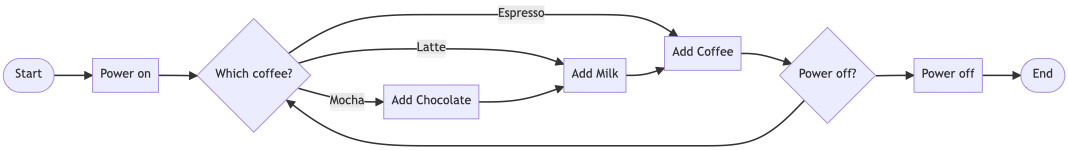
\includegraphics[width=1.0\textwidth]{images/coffee-flow.png}

  \doExercise{Write the process of the flowchart above}{
        $P ~~=~ \mf{powerOn} . Q$\\
        $Q ~~=~ \mf{selMocha}.\mf{addChocolate}.Mk + \mf{selLatte}.Mk + \ldots $\\
        $Mk ~=~ \mf{addMilk}\ldots$  
      ~\\[0.35\textheight]
  }

\end{slide}



% ----------------------------------------

\section{Concurrent Process algebra}


\begin{slide}{Overview}

\begin{block}{Recall}
\begin{enumerate}
  \item Non-deterministic Finite Automata ($X \to \faded{\mathtt{Bool}} \times \mathtt{P}(X)^{\Act}$):
  \wrap{\small\begin{tikzpicture}[aut]
  \node[st,initial]  (q1) {$q_1$};
  \node[st,final] (q2) [right of=q1]  {$q_2$};
  \path[->] (q1) edge node {a} (q2) (q2) edge[loop right] node {b} ();
\end{tikzpicture}}
  \item (Sequential) Process algebra:
    $P = a.Q ~~~~ Q=b.Q$

  \item Meaning of \structure{(2)} using \structure{(1)}
\end{enumerate}  
\end{block}

\begin{block}{Still missing}
\begin{itemize}
  \item \alert{\textbf{Interaction}} between processes
  % \item \emph{Interaction \alert{diagrams}} vs. \emph{interacting \alert{processes}}
  \item Enrich \structure{(2)} and \structure{(3)}
\end{itemize}
\end{block}

\end{slide}

%-------------------------------------------------------------------------------
\begin{slide}{Process algebras}
\small

\begin{block}{CCS - \alert{Updated} Syntax}
\begin{equation*}
% \mathcal{P} ~\ni~ P,Q\; ::=\; K ~~|~~ \alpha.P ~~|~~ \sum_{i\in I} P_i
%         ~~|~~ \crn P f \transp{~~|~~ P|Q ~~|~~ P\backslash L}
\mathcal{P} ~\ni~ P,Q\; ::=\; K ~~|~~ \alpha.P ~~|~~ P + Q ~~|~~ \cnil
        ~~|~~ \crn P f  ~~|~~ P\backslash L ~~|~~ \alert{P|Q}
\end{equation*}
%
where
\\- $\alpha \in \Act \alert{\cup \overline\Act}
    \cup \set{\tau}$~ is an action
\\- $K$ s a collection of process names or process constants
\\- $L \subseteq \Act %\transp{\cup \overline{\Act}}
    $ is a set of labels
\\- $f$ is a function that renames actions s.t. $f(\tau) = \tau$  \alert{and $f(\overline{a}) = \overline{f(a)}$}
\\- notation:
% \\~~~~~$\cnil = \sum_{i\in\emptyset}P_i$
% \\~~~~~$P_1+P_2 = \sum_{i\in\set{1,2}}P_i$
\\~~~~~$[f] = [a_1\mapsto b_1,\ldots,a_n \mapsto b_n]$~~~~~where \alert{$a_i,b_i \in N \cup \set{\tau}$}
\end{block}
\end{slide}

%-------------------------------------------------------------------------------

\begin{slide}{Process algebras}
\small

\begin{block}{Syntax}
\begin{equation*}
% \mathcal{P} ~\ni~ P,Q\; ::=\; K ~~|~~ \alpha.P ~~|~~ \sum_{i\in I} P_i
%         ~~|~~ \crn P f \transp{~~|~~ P|Q ~~|~~ P\backslash L}
\mathcal{P} ~\ni~ P,Q\; ::=\; K ~~|~~ \alpha.P ~~|~~ P + Q ~~|~~ \cnil
        ~~|~~ \crn P f  ~~|~~ P\backslash L ~~|~~  \alert{P|Q}
\end{equation*}
\end{block}

%\setcounter{equation}{0}
\begin{exampleblock}{\exercise Which are syntactically correct?}
\begin{columns}
  \column{0.38\textwidth}
  \begin{align}
    & a.\ainv b.A+B\\&
    (a.\cnil + \ainv a.A) \backslash \set{\ainv{a},b}\\&
    (a.\cnil + \ainv a.A) \backslash \set{a,\tau}\\& % no
    (a.\cnil + \ainv{\tau}.A) \backslash \set{a}\\& % no
    % a.B+[b\mapsto a]\\& % no
    \tau.\tau.B + \ainv a.\cnil %\\&
    % a.(a + b).A
    \\&
    (\cnil | \cnil) + \cnil
  \end{align}

  \column{0.45\textwidth}
  \begin{align} &
    (a.B + b.B)[a\mapsto a,\tau\mapsto b]\\&
    (a.B + \tau.B)[b\mapsto a,b\mapsto a]\\& % no
    (a.B + b.B)[a\mapsto b,b\mapsto \ainv a]\\& % no
    (a.b.A + \ainv a.\cnil)|B\\&
    (a.b.A + \ainv a.\cnil).B\\&
    (a.b.A + \ainv a.\cnil)+B
  \end{align}
\end{columns}
\end{exampleblock}

\end{slide}

%-------------------------------------------------------------------------------

\begin{slide}{CCS semantics - building an NFA}
\small 
\centering
\newcommand{\msep}{~~~~~~}
\vspace*{-2mm}

\typerule{act}{\shrk}{\alpha.P \trans\alpha P}
\msep
\typerule{sum-1}{P_1 \trans\alpha P'_1}{P_1 + P_2 \trans\alpha P'_1} %$\transp{j\in I}$
\msep
\typerule{sum-2}{P_2 \trans\alpha P'_2}{P_1 + P_2 \trans\alpha P'_2} %$\transp{j\in I}$
\\[2mm]
\typerule{res}{P\trans\alpha P'}{\crt P L\trans\alpha \crt{P'}L}~$\transp{\alpha,\ainv{\alpha}
                                                                  \notin L}$
\msep
\typerule{rel}{P\trans\alpha P'}{\crn P f\trans{f(\alpha)} \crn{P'} f}
\\[2mm]
\alert{
\typerule{com1}{P\trans\alpha P'}{P|Q\trans\alpha P'|Q}
\msep
\typerule{com2}{Q\trans\alpha Q'}{P|Q\trans\alpha P|Q'}
\msep
\typerule{com3}{P\trans a P' \quad Q\trans{\ainv{a}} Q'}{P|Q\trans\tau P'|Q'}
}
\\[2mm]
\pause

\begin{exampleblock}{\exercise Draw the transition systems}
  \exerciseBack
  \vspace*{-5mm}
  \begin{align*}
    % CM &= \mathsf{coin.coffee}.CM
    % \\
    % CS &= \mathsf{pub.(coin.coffee.CS + coin.tea.CS)}
    CM &= \mathsf{coin.\ainv{coffee}}.CM
    \\
    CS &= \mathsf{pub.\ainv{coin}.coffee}.CS
    \\
    SmUni &= \crt{(CM|CS)}{\mathsf{\set{coin,coffee}}}
  \end{align*}
  \vspace*{-7mm}
\end{exampleblock}
\end{slide}
\exerciseAdd



\begin{slide}{Exercises}
  \doExercise{Let $A=b.a.B$. Show that:}{
    \vspace*{-8mm}
    \begin{enumerate}
      \item $(A ~|~ \overline{b}.\cnil)\backslash \{b\}~\trans\tau~ (a.B ~|~ \cnil)\backslash\{b\}$
      \item $(A ~|~ b.a.B) + ((b.A)[b\mapsto a]) ~\trans{a}~ A[b \mapsto a]$
    \end{enumerate}
  }  

  \doExercise{Draw the NFAs $A$ and $D$}{
    \vspace*{-8mm}

    \begin{columns}
    \col[0.45]{      
    \begin{align*}
      A &= x.B+x.x.C\\
      B &= x.x.A+y.C\\
      C &= x.A      
    \end{align*}
    }
    \col[0.45]{      
    \begin{align*}
      D &= x.x.x.D + x.E\\
      E &= x.F+y.F\\
      F &= x.A      
    \end{align*}
    }
    \end{columns}
  }  

\end{slide}


\section{Observational Equivalence}

\begin{slide}{Overview}

\begin{block}{Recall}
\begin{enumerate}
  \item F-transition systems, e.g., Non-deterministic Finite Automata:
  \wrap{\small\begin{tikzpicture}[aut]
  \node[st,initial]  (q1) {$q_1$};
  \node[st,final] (q2) [right of=q1]  {$q_2$};
  \path[->] (q1) edge node {a} (q2) (q2) edge[loop right] node {b} ();
\end{tikzpicture}}
  \item Process algebra:
    $P = a.Q ~~~~ Q=b.Q ~~~~ P|Q$

  \item Interaction between processes
  
  \item Meaning of CCS using transition systems

  % \item Equivalence relations ((bi)simulations)
\end{enumerate}  
\end{block}

\begin{block}{Still missing}
\begin{itemize}
  \item When is a process $P$ \alert{equivalent} to a process $Q$?
  \item When can a process $P$ be \alert{safely replaced} by a process $Q$?
  % \item When can a sequence of interactions be \alert{safely implemented} as interacting components?
\end{itemize}
\end{block}
\end{slide}


\begin{frame}{Observational Equivalence Informally}

  Two programs are \structure{observationally equivalent} if it is impossible to \alert{observe any
  difference} in their \alert{behaviour}

  
  \vfill
  Here behaviour is described in terms of transition systems

  \dots\ and therefore behaviour/equivalence needs to be pinned
  down to them
\end{frame}

\section{EQ1 -- Language equivalence}

%----------------------------------------------------------------------------------
\begin{slide}{Language  equivalence}
\small

\begin{block}{Definition}
Two automata $A, B$ are \alert{language equivalent} iff  $ L_A =  L_B$\\
(i.e. if they can perform the same finite sequences of transitions)
\end{block}
~\\

\begin{example}
  \centering
  % Requires \usepackage{graphicx}
  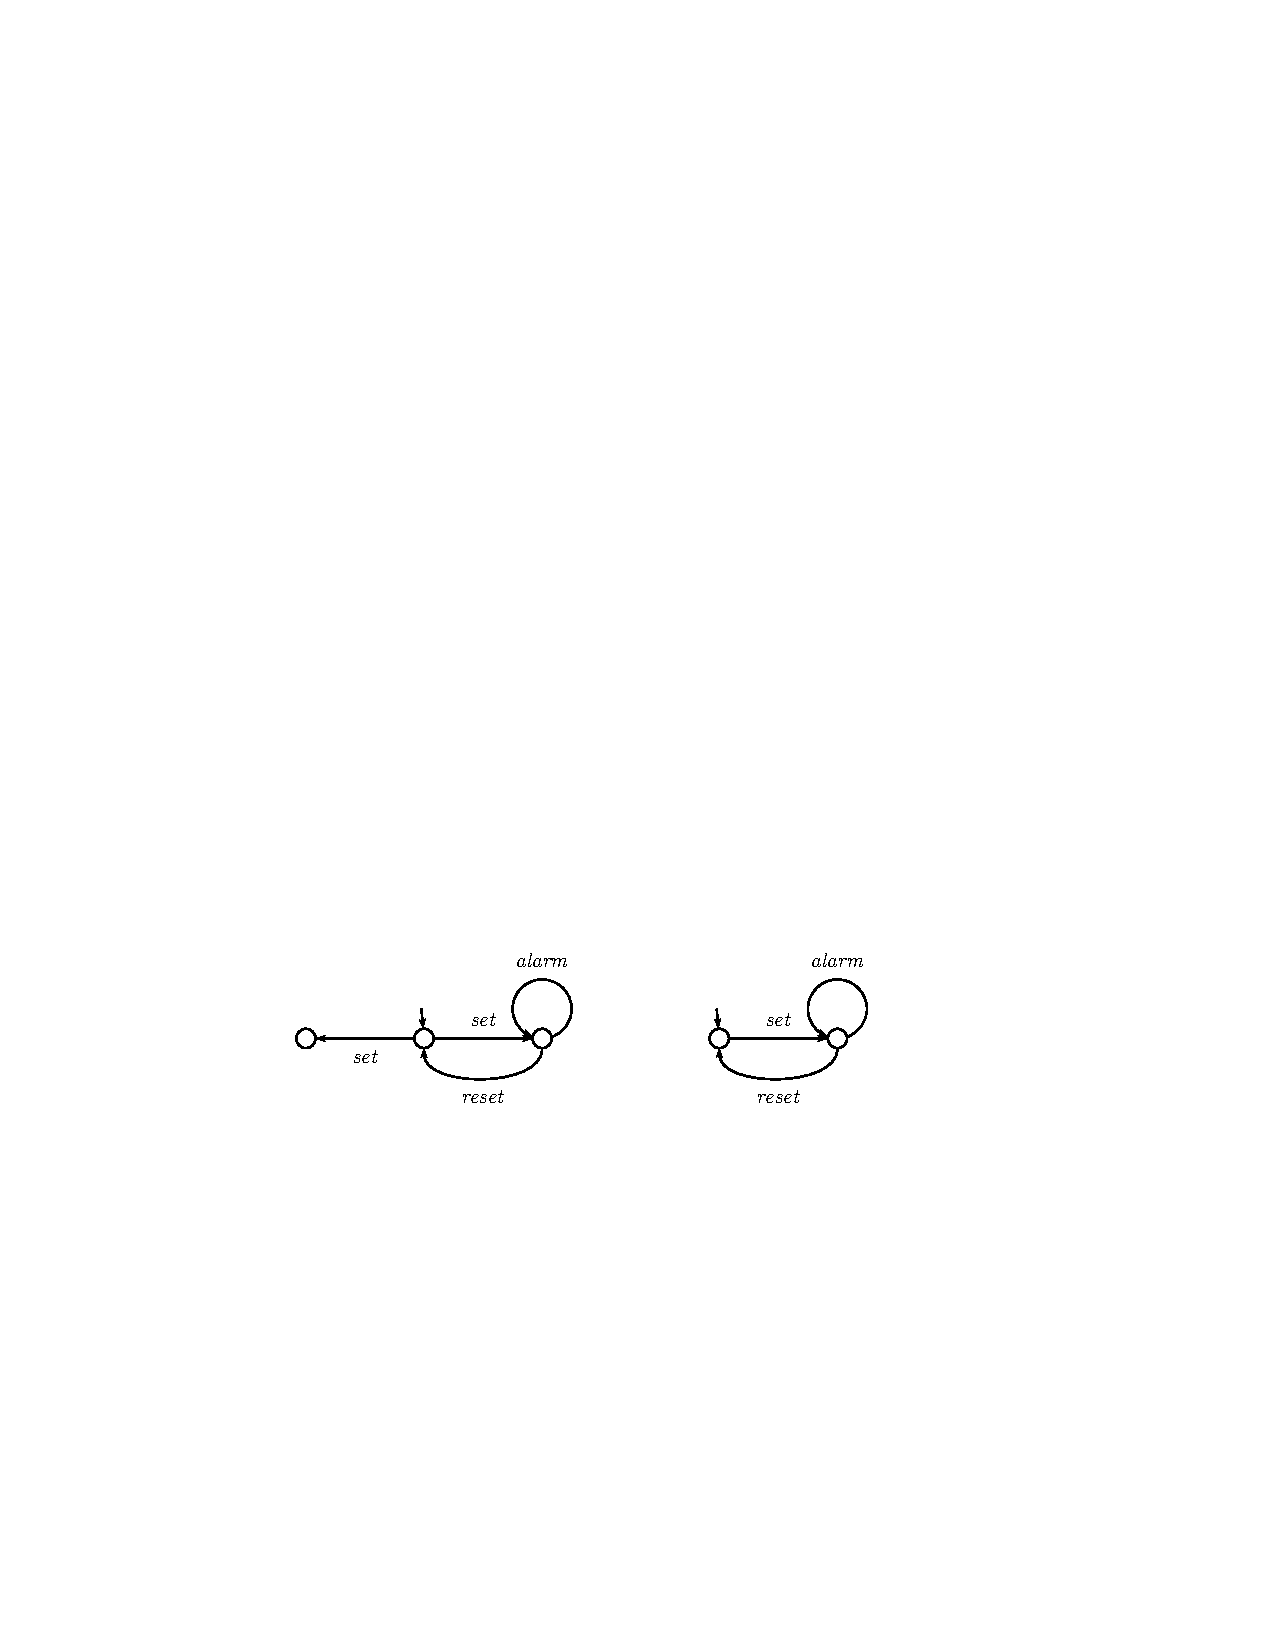
\includegraphics[width=9cm]{./images/alarm3.pdf}
\end{example}


\alert{Language equivalence} applies  when one can neither interact with a system, nor distinguish a slow system from one that has come to a stand still.
\end{slide}


% \begin{slide}{Exercise}
%   \centering
%   \doExercise{Consider the system}{
%   \centering
%   \begin{tikzpicture}
%       \node(p){$p$}; \node[right=of p](p1){$p_1$}; \node[right=of p1](p2){$p_2$};
%       \draw[->] (p)edge[bend right] node[below]{a} (p1)
%                 (p1)edge[bend right] node[above]{b}(p)
%                 (p2)edge node[above]{d} (p1)edge[loop right] node[right]{c}(p1) ;
%   \end{tikzpicture}
%   \begin{enumerate}
%     \item Formalise the system as a tuple $(S,Act,\to)$
%     \item List 4 different traces from state (p2).
%   \end{enumerate}
%   }
% \end{slide}


\begin{slide}{Exercise}
  \centering
  \doExercise{Find pairs of automata with the same language}{
    \centering 
    \wrap{\begin{tikzpicture}[aut]
      \node[st,initial above,final]  (s_0) {$A_0$};
      \node[st] (s_1) [right of=s_0] {$A_1$};
      \path[->]
        (s_0) edge  node {a}  (s_1)
        (s_0) edge[loop left] node {a}  ()
        (s_1) edge[loop right] node {b}  (s_0);
    \end{tikzpicture}}
    ~~~~~~~~~~
    \wrap{\begin{tikzpicture}[aut]
      \node[st,initial above,final]  (s_0) {$B_0$};
      \node[st,final] (s_1) [right of=s_0] {$B_1$};
      \path[->]
        (s_0) edge  node {a}  (s_1)
        (s_0) edge[loop left] node {a}  ()
        (s_1) edge[loop right] node {a}  (s_0);
    \end{tikzpicture}}
    ~~~~~~~~~
    \wrap{\begin{tikzpicture}[aut]
      \node[st,initial above]  (s_0) {$C_0$};
      \node[st,final] (s_1) [right of=s_0] {$C_1$};
      \path[->]
        (s_0) edge  node {a}  (s_1)
        (s_0) edge[loop left] node {a}  ()
        (s_1) edge[loop right] node {b}  (s_0);
    \end{tikzpicture}}
    ~~~~~~~~~
    \wrap{\begin{tikzpicture}[aut]
      \node[st,initial above]  (s_0) {$D_0$};
      \node[st,final] (s_1) [right of=s_0] {$D_1$};
      \path[->]
        (s_0) edge  node {a}  (s_1)
        (s_0) edge[loop left] node {a}  ()
        (s_1) edge[loop right] node {a}  (s_0);
    \end{tikzpicture}}
    ~~~~~~~~~
    \wrap{\begin{tikzpicture}[aut]
      \node[st,initial above]  (s_0) {$E_0$};
      \node[st,final] (s_1) [right of=s_0] {$E_1$};
      \path[->]
        (s_0) edge[bend left]  node {a}  (s_1)
        (s_1) edge[bend left]  node {a}  (s_0)
        (s_1) edge[loop right] node {a}  (s_0);
    \end{tikzpicture}}

  }
\end{slide}

\begin{slide}{Exercise}
  \doExercise{Check if the processes are language equivalent}{
    \begin{align*}
      P &= coin.(\ainv{coffee}.P + \ainv{tea}.P)
      &
      Q &= coin.\ainv{coffee}.Q + coin.\ainv{tea}.Q
    \end{align*}
  }

\end{slide}


\section{EQ2 -- Similarity}

%----------------------------------------------------------------------------------
\begin{slide}{Simulation}
\begin{flushright}
the quest for a \alert{behavioural equality}:\\
able to identify states that cannot be distinguished by any \alert{realistic} form of  observation
\end{flushright}
~\\

\small
\begin{block}{Simulation}
% \caixa
{A state $q$ \alert{simulates} another state $p$
\alert{if}\\
every transition from $q$ is corresponded by a transition from $p$
\alert{and}\\
this capacity is kept along the whole life of the system to which state space $q$ belongs to.}
\end{block}
\end{slide}

%----------------------------------------------------------------------------------
\begin{slide}{Simulation of NFA ($X \to \mathtt{P}(X)^{\Act}$)}
\small

\begin{block}{Definition}
% Given  $\pair{S_1, \Act, \rra_1}$  and $\pair{S_2, \Act, \rra_2}$
%  over $\Act$ \faded{(ignoring initial and final states)}
Given NFA $A_1$ and $A_2$ over \Act\ with states $S_1$ and $S_2$ respectively,
a relation \structure{$R \subseteq S_1 \times S_2$} is a \structure{simulation} iff,
for all $\pair{p,q} \in \structure{R}$ and $a \in \Act$,

\begin{align*}
%\text{\gold{(1)}}\; \;  & p \downarrow_1 \;  \imp\; q \downarrow_2\\ &\\
\text{\alert{(1)}}\; \;  & p \rtran{a}_1 p'\;  \imp\; \rcb{\exists}{q'}{q' \in S_2}{q \rtran{a}_2 q'\, \land\, \pair{p',q'} \in \structure{R}}   
\end{align*}
\vspace{0mm}

\begin{equation*}
\xymatrix{
p \ar[d]^-{a} & \hspace{-1.5cm} \structure{R}  & \hspace{-2.7cm} q 
  & \!\! \text{\raisebox{-10mm}{\Huge $\imp$}} \! \! &  &  &  q \ar[d]^-{a} \\
p'           &   &           &                                   & p'\hspace{-2.7cm} &  \structure{R} \hspace{-1.5cm} &  q'
}
\end{equation*}

\end{block}
\end{slide}

%----------------------------------------------------------------------------------
\begin{slide}{Example}

\begin{exampleblock}{\exercise Find simulations}
\begin{equation*}
\xymatrix{
& q_1  \ar[r]^{d} & q_2 &       &        &                              p_2\\
q_0 \ar[ru]^{a} \ar[rd]_{a} &  & & p_0 \ar[r]^{a} & p_1 \ar[ru]^{d} \ar[rd]_{e} & \\
& q_4  \ar[r]_{e} & q_3 &       &        &                              p_3\\
}
\end{equation*}
\end{exampleblock}

\vspace{0.2cm}
\visible<2->{\exerciseBack\begin{equation*}
q_0 \lesssim p_0 \text{\hspace{0.5cm} cf. \hspace{0.3cm}} 
\set{\pair{q_0,p_0}, \pair{q_1,p_1},\pair{q_4,p_1},\alert{\ldots}} %\pair{q_2,p_2},\pair{q_3,p_3}}
\end{equation*}}
\end{slide}

\exerciseAdd


%----------------------------------------------------------------------------------
\begin{slide}{Similarity}
\small

\begin{block}{Definition}
\centering
\[p \lesssim q\; \equiv\; \rcb{\exists}{R}{}{R\; \text{is a simulation and}\; \pair{p,q} \in R} 
\]
\emph{We say \alert{$p$ is simulated by $q$}.}
\end{block}

% \begin{block}{Automata simulation}
%   \[\pair{S_1,\set{s_1},\dda_1,\rra_1} \lesssim \pair{S_2,\set{s_2},\dda_2,\rra_2}\; \equiv\; s_1 \lesssim s_2 
% \]
% \end{block}

\begin{block}{Lemma}
The similarity relation is a preorder\\
\faded{(ie, reflexive and transitive)}
\end{block}
\end{slide}



%-------------------------

\section{EQ3 -- Bisimilarity}
%----------------------------------------------------------------------------------
\begin{slide}{Bisimulation}
\small

\begin{block}{Definition}
% Given  $\pair{S_1, \Act,  \rra_1}$  and $\pair{S_2, \Act, \rra_2}$ over $\Act$,
Given NFA $A_1$ and $A_2$ over \Act\ with states $S_1$ and $S_2$ respectively,
relation $R \subseteq S_1 \times S_2$ is a \structure{bisimulation} iff both $R$ and its converse $\aconv{R}$
are simulations.

I.e.,
whenever $\pair{p,q} \in R$ and $a \in \Act$,

\begin{align*}
%\text{\gold{(1)}}\; \;  &  p \downarrow_1 \;  \dimp\; q \downarrow_2\\ &\\
\text{\alert{(1)}}\; \;  & p \rtran{a}_1 p'\; \imp\; \rcb{\exists}{q'}{q' \in S_2}{q \rtran{a}_2 q'\, \land\, \pair{p',q'} \in R}   \\
\text{\alert{(2)}}\; \;  & q \rtran{a}_2 q'\; \imp\; \rcb{\exists}{p'}{p' \in S_1}{p \rtran{a}_1 p'\, \land\, \pair{p',q'} \in R}   
\end{align*}

%\begin{equation*}
%\xymatrix{
%p \ar[d]^-{a} & \hspace{-1.5cm} R  & \hspace{-2.7cm} q
%    & \! \! \text{\raisebox{-10mm}{\Huge $\Leftrightarrow$}} \! \! &   &  
%    &  q \ar[d]^-{a} \\
%p'           &   &           &                                   & p'\hspace{-2.7cm} &  R \hspace{-1.5cm} &  q'
%}
%\end{equation*}
\centering
\begin{tikzpicture}[%
    every edge/.style={draw, thick,-latex',shorten >= 2pt}]
  \tikzstyle{l} = [auto,inner sep=1pt]
  % the square
  \node(p){$p$};\node[right=2.3 of p](q2){$q$};
  \node[below=1 of p](p'){$p'$};\node(q')at(p'-|q2){$q'$};
  % the R parts
  \node[right=0 of p](R1){$R$};\node[right=0 of R1](q){$q$};
  \node[left=0 of q'](R2){$R$};\node[left=0 of R2](p'2){$p'$};
  % the arrows
  \draw[->] (p)edge node[l]{$a$}(p') (q2)edge node[l]{$a$}(q');
  \node at ($(p)!.5!(q')$){{\Large $\Rightarrow$}};
  %%%%%%%
  % the square
  \node[right=2.3 of q2](pp){$p$};\node[right=2.3 of pp](q2){$q$};
  \node[below=1 of pp](p'){$p'$};\node(q')at(p'-|q2){$q'$};
  % the R parts
  \node[right=0 of p'](R1){$R$};\node[right=0 of R1](q){$q'$};
  \node[left=0 of q2](R2){$R$};\node[left=0 of R2](p'2){$p$};
  % the arrows
  \draw[->] (pp)edge node[l]{$a$}(p') (q2)edge node[l]{$a$}(q');
  \node at ($(pp)!.5!(q')$){{\Large $\Leftarrow$}};

\end{tikzpicture}

\end{block}
\end{slide}



%----------------------------------------------------------------------------------
\begin{slide}{Examples}

\doExercise{Find bisimulations that include $\pair{q_1,m}$}{
\begin{equation*}
\xymatrix{
& q_1  \ar[ld]_{a}  \ar[rd]^{a} & & & & m \ar[d]_{a}\\
q_2 \ar[rr]^{c}  && q_3 \ar@(ur,dr)[]^{c}  & & & n\ar@(ur,dr)[]^{c}
}
\end{equation*}
% R = \enset{(q_1,m), (q_2, n), (q_3,n) }
}

\doExercise{Find bisimulations that include $\pair{q_1,h}$}{

\begin{equation*}
\xymatrix{
q_1 \ar[r]^{a} & q_2  \ar[r]^{a}  & q_3  \ar[r]^{a} & \cdots & & h\ar@(ur,dr)[]^{a}  \\
}
\end{equation*}
% R = \setdef{q_i, h}{i \geq 1}  
}

\end{slide}


%----------------------------------------------------------------------------------
\begin{slide}{Exercises}

\doExercise{Check if there is a bisimulation that include $\pair{q_1,p_1}$}{
\vspace*{-3mm}
\begin{equation*}
\xymatrix{
& q_1  \ar[ld]_{a}  \ar[rd]^{a} & & & & p_1  \ar[d]^{a} \\
q_2 \ar[d]^{c}  && q_3  \ar[d]^{c}  & && p_2  \ar[ld]_{c}  \ar[rd]^{c} & \\
q_4 & & q_5 & &p_4 & & p_5\\
% & q_1  \ar[ld]_{a}  \ar[rd]^{a} & & & & p_1  \ar[d]^{a} \\
% q_2 \ar[d]^{\rdb{b}}  && q_3  \ar[d]^{c}  & && p_2  \ar[ld]_{\rdb{b}}  \ar[rd]^{c} & \\
% q_4 & & q_5 & &p_4 & & p_5
}
\end{equation*}
}
\end{slide}


\begin{slide}{Exercises}
\doExercise{Check if there is a bisimulation that include $\pair{q_1,p_1}$}{
\vspace*{-3mm}
\begin{equation*}
\xymatrix{
% & q_1  \ar[ld]_{a}  \ar[rd]^{a} & & & & p_1  \ar[d]^{a} \\
% q_2 \ar[d]^{c}  && q_3  \ar[d]^{c}  & && p_2  \ar[ld]_{c}  \ar[rd]^{c} & \\
% q_4 & & q_5 & &p_4 & & p_5\\
& q_1  \ar[ld]_{a}  \ar[rd]^{a} & & & & p_1  \ar[d]^{a} \\
q_2 \ar[d]^{\rdb{b}}  && q_3  \ar[d]^{c}  & && p_2  \ar[ld]_{\rdb{b}}  \ar[rd]^{c} & \\
q_4 & & q_5 & &p_4 & & p_5
}  
\end{equation*}
}

\doExercise{Check if there is a bisimulation that include $\pair{P,Q}$}{
  \vspace*{-5mm}
  \begin{align*}
      P &= coin.(\ainv{coffee}.P + \ainv{tea}.P)
      &
      Q &= coin.\ainv{coffee}.Q + coin.\ainv{tea}.Q
  \end{align*}
}

\end{slide}



% Definition
% p∼q ≡ ⟨∃R :: Risabisimulationand⟨p,q⟩∈R⟩
%----------------------------------------------------------------------------------
\begin{slide}{Bisimilarity}
\small

\begin{block}{Definition}
\centering
\[p \sim q\; \equiv\; \rcb{\exists}{R}{}{R\; \text{is a bisimulation and}\; \pair{p,q} \in R} 
\]
\emph{We say \alert{$p$ is bisimilar to $q$}.}
\end{block}


\begin{block}{Lemma}
\centering
Two processes $P$ and $Q$ are bisimilar if there is a bisimulation that includes $\pair{P,Q}$.
\end{block}

\begin{block}{Lemma}
The bisimilarity relation is an equivalence relation\\
\faded{(ie, symmetric, reflexive and transitive)}
\end{block}


% \begin{block}{Automata simulation}
%   \[\pair{S_1,\set{s_1},\dda_1,\rra_1} \lesssim \pair{S_2,\set{s_2},\dda_2,\rra_2}\; \equiv\; s_1 \lesssim s_2 
% \]
% \end{block}

% \begin{block}{Lemma}
% The similarity relation is a preorder\\
% \faded{(ie, reflexive and transitive)}
% \end{block}
\end{slide}



\section{Generalising Observational Equivalences}

\begin{frame}{$F$-Transition Systems and Observational \underline{Equivalence}}

  \begin{definition}
    Fix a functor $F$ and consider two transition systems
    $f : X \to F X$ and $g : Y \to F Y$. Two states $x \in X$, $y \in Y$
    are observationally equivalent if there exists a relation
    $R \subseteq X \times Y$ with $(x,y) \in R$ and there exists a
    transition system $b : R \to FR$ such that the diagram below commutes
    \[
      \xymatrix{
        X \ar[d]_{f} & \ar[l]_{\pi_1}  R \ar[r]^{\pi_2} \ar[d]_{b} & Y \ar[d]^{g} \\
        F X  & \ar[l]^{F \pi_1} FR \ar[r]_{F \pi_2} & F Y
        }
    \]
    If such is the case we write \alert{$x \sim y$}  
  \end{definition}
\end{frame}

\begin{frame}{Observational Equivalence for Moore Automata}
  Given $\pv{o_1}{n_1} : X \to A \times X$ and
  $\pv{o_2}{n_2} : Y \to A \times Y$ we obtain from the previous slide 
  that $x \sim y$ iff
  \begin{itemize}
  \item $o_1(x) = o_2(y)$
  \item $n_1(x) \sim n_2(y)$
  \end{itemize}
\end{frame}

\begin{frame}{Observational Equivalence for Labelled Transition Systems}
  Recall that we used systems of type $X \to \Pow(X)^L$ for establishing the
  \alert{semantics} of \alert{CCS processes}. This means that \dots

  notions of observational behaviour/equivalence for such transition systems
  directly impact our concurrent language

  \vfill Given $\overline{t_1} : X \to \Pow(X)^L$ and
  $\overline{t_2} : Y \to \Pow(Y)^L$, $x \sim y$ iff for all $l \in L$
  \begin{itemize}
  \item $\forall x' \in t_1(x,l).\  \exists y' \in t_2(y,l).\ x' \sim y'$
  \item $\forall y' \in t_2(y,l).\ \exists x' \in t_1(x,l).\ x' \sim y'$
  \end{itemize}
\end{frame}


% \begin{frame}{Is Observational Equivalence a Good Notion of Equivalence?}

%   \begin{block}{Coinduction Principle}
%       Two states $x,y$ are observationally \alert{equivalent} iff they produce the
%       \alert{same} observational behaviour
%   \end{block}
  
% \end{frame}

\end{document}
